% Welcome! This is the unofficial University of Udine beamer template.

% See README.md for more informations about this template.

% This style has been developed following the "Manuale di Stile"
% (Style Manual) of the University of Udine. You can find the
% manual here: https://www.uniud.it/it/ateneo-uniud/ateneo-uniud/identita-visiva/manuali-immagine-stile/manuale-stile

% Note: for some reason, the RGB values specified in the manual
% do NOT render correctly in Beamer, so they have been redefined
% for this document using the high level chromo-optic deep neural 
% quantistic technology offered by Microsoft Paint's color picker.

% We defined four theme colors: UniBrown, UniBlue, UniGold
% and UniOrange. For example, to write some uniud-brownish
% text, just use: \textcolor{UniBrown}{Hello!}

% Note that [usenames,dvipsnames] is MANDATORY due to compatibility
% issues between Madrtikz and xcolor packages.

\documentclass[usenames,dvipsnames]{beamer}
\usepackage[utf8]{inputenc}
\usepackage{verbatim}
%\usetheme{uniud}
\usetheme[progressbar=frametitle]{Boadilla}
\usecolortheme{dove}
\addtobeamertemplate{footnote}{\vspace{-6pt}\advance\hsize-0.5cm}{\vspace{6pt}}
\usepackage{amsmath,amssymb}
\usepackage{graphicx}
\usepackage{color}
\usepackage{setspace}
\usepackage[english]{babel}
\usepackage[utf8]{inputenc}
\usepackage{times}
\usepackage{tikz}
\usepackage{lipsum}%
\usepackage{amsmath}
\usepackage{lastpage}
\usepackage{verbatim}
\usetikzlibrary{calc,arrows,shapes,positioning}
\usepackage{color,soul}
\usepackage{booktabs }
\usepackage{algorithm,algorithmic}
\usepackage{tikz,pgfplots}
\usepackage{mathptmx}
\usepackage[scaled=.90]{helvet}
\usepackage{courier}
\usepackage[absolute,overlay]{textpos}
\usepackage{graphicx}
\usepackage{booktabs}
\usepackage{units}
\usepackage{subfigure}
\usepackage{float}
\usepackage{array}
\usepackage{environ}
\usepackage{esint}
\usepackage{hyperref}
\usepackage{ragged2e}
\usepackage[autoplay,autoresume]{animate}
\usepackage[font={small,it}]{caption}
 \usepackage{subfigure} % subfiguras
\usepackage{lipsum}% http://ctan.org/pkg/lipsum
\usepackage{hanging}% http://ctan.org/pkg/hanging
\usepackage[style=authoryear,backend=biber]{biblatex}
\usepackage{pgfplots}
\usepackage{footmisc}
\usepackage{etoolbox}
\usepackage{tikz}
\usetikzlibrary{backgrounds,shapes.multipart}
\pgfdeclarelayer{myback}
\pgfsetlayers{background,main,myback} %<= insert the myback 
% after the "main" to display the content in front of the usual content
\usepackage{lipsum} % <= to insert dummy text
\usepackage[absolute,overlay]{textpos}
% definition of the style
\tikzset{exampleblock/.style={rounded corners,rectangle split, rectangle split parts=2, draw, 
rectangle split part fill={green!80!black, green!20},minimum width=\textwidth
}}

\usepackage{lipsum} 

\addbibresource{bibliography.bib}

\BeforeBeginEnvironment{theorem}{
    \setbeamercolor{block title}{fg=black,bg=orange!50!white}
    \setbeamercolor{block body}{fg=orange, bg=orange!30!white}
}
\AfterEndEnvironment{theorem}{
 \setbeamercolor{block title}{use=structure,fg=structure.fg,bg=structure.fg!20!bg}
 \setbeamercolor{block body}{parent=normal text,use=block title,bg=block title.bg!50!bg, fg=black}
}
%%% Suppress biblatex annoying warning
\usepackage{silence}
\WarningFilter{biblatex}{Patching footnotes failed}

%%% Some useful commands
% pdf-friendly newline in links
\newcommand{\pdfnewline}{\texorpdfstring{\newline}{ }} 
% Fill the vertical space in a slide (to put text at the bottom)
%\newcommand{\framefill}{\vskip0pt plus 1filll}

\usepackage{lipsum}% http://ctan.org/pkg/lipsum
\usepackage{hanging}% http://ctan.org/pkg/hanging

\let\oldfootnote\footnote
\renewcommand\footnote[1][]{\footnotesize\oldfootnote[frame,#1]}
\renewcommand{\footnotesize}{\tiny}
\renewcommand{\footnoterule}{%
\kern 2pt
}

\definecolor{UniRed}{RGB}{166,28,49}

\setbeamertemplate{section page}
{
    \begingroup
    \begin{beamercolorbox}[sep=18pt,center]{section title}
        \usebeamerfont{section title}\insertsection\par
    \end{beamercolorbox}
    \endgroup
}
% Add support for \subsubsectionpage
\def\subsubsectionname{\translate{Subsubsection}}
\def\insertsubsubsectionnumber{\arabic{subsubsection}}
\setbeamertemplate{subsubsection page}
{
%  \begin{centering}
%    {\usebeamerfont{subsubsection name}\usebeamercolor[fg]{subsubsection name}\subsubsectionname~\insertsubsubsectionnumber}
%    \vskip1em\par
%    \begin{beamercolorbox}[sep=4pt,center]{part title}
%      \usebeamerfont{subsubsection title}\insertsubsubsection\par
%    \end{beamercolorbox}
%  \end{centering}
}
\def\subsubsectionpage{\usebeamertemplate*{subsubsection page}}

\AtBeginSection{\frame{\sectionpage}}
\AtBeginSubsection{\frame{\subsectionpage}}
\AtBeginSubsubsection{\frame{\subsubsectionpage}}







\makeatother
\setbeamertemplate{footline}
{
  \leavevmode%
  \hbox{%
  \begin{beamercolorbox}[wd=2.0\paperwidth,ht=2.25ex,dp=1ex,center]{}%
    \insertframenumber{} / \inserttotalframenumber\hspace*{1ex}
  \end{beamercolorbox}}%
  \vskip0pt%
}

\newcommand\blfootnote[1]{%
  \begingroup
  \renewcommand\thefootnote{}\footnote{#1}%
  \addtocounter{footnote}{-1}%
  \endgroup
}










\PassOptionsToPackage{demo}{graphicx}

\makeatletter
\newcommand\titlegraphicii[1]{\def\inserttitlegraphicii{#1}}
\titlegraphicii{}
\setbeamertemplate{title page}
{
  
  \begin{centering}
    \begin{beamercolorbox}[sep=8pt,center]{institute}
      \usebeamerfont{institute}\insertinstitute
    \end{beamercolorbox}
    \begin{beamercolorbox}[sep=8pt,center]{title}
      \usebeamerfont{title}\inserttitle\par%
      \ifx\insertsubtitle\@empty%
      \else%
        \vskip0.25em%
        {\usebeamerfont{subtitle}\usebeamercolor[fg]{subtitle}\insertsubtitle\par}%
      \fi%     
    \end{beamercolorbox}%
    \vskip1em\par
    \begin{beamercolorbox}[sep=8pt,center]{date}
      \usebeamerfont{date}\insertdate
    \end{beamercolorbox}%\vskip0.5em
    \begin{beamercolorbox}[sep=8pt,center]{author}
      \usebeamerfont{author}\insertauthor
    \end{beamercolorbox}
  \end{centering}
 % \vbox{}
   {\usebeamercolor[fg]{titlegraphic}\inserttitlegraphic\hfill\inserttitlegraphicii\par}
  %\vfill
}
\makeatother
\author{M.Sc. Ricardo Moncayo, Ph.D. Anne Martel, Ph.D. Eduardo Romero}
\title{Breast Cancer Recurrence Prediction using a Quantitative Evaluation of the Nuclear Pleomorphism}
%\subtitle{Presentation Subtile}
\institute{Department of \\
Electrical Engineering}
\date{\today}
\titlegraphic{\Centering\includegraphics[height=0.35\textheight]{graphics/cabeza.png}}
%\titlegraphicii{\includegraphics[height=2.5cm,width=2.5cm]{graphics/logo.png}}



\begin{document}

\begin{frame}[plain]
\maketitle
\small
{\centering\itshape \par}
\par\medskip

\end{frame}

%%%%%%%%%%%%%%%%%%%%%%%%%%%%%%%%%%%%%%%%%%%%%%%%%%%%%%%%%%%%%

% \begin{frame}{Pathological examination issues}
% 	\begin{itemize}
% 	 \item  Diagnosis is not quantified from tumour tissue since this is highly variable 
%      \pause
% 	 \item Observations depend on inter and intra observer variations
%       %\textcolor{red}{Imagenes con kappa}	 
	 
% 	% \item As consequence the prognosis is prone to error
% 	 % tumor contour, lymphotic reaction in tumor, nuclear cytology, vascular invasion, tumor proliferation
% 	\end{itemize}
% \end{frame}

% \begin{frame}{ Suitability of  Quantitative Estimation in Pathology Workflow}
%  \begin{itemize}
%   \item Digital  whole glass slides  are being used to quantify  diagnosis
%   \pause

%   \item  Quantification of  structures may help to determine predisposition to a disease %\textcolor{red}{imagenes??}
  
  
  
%  \end{itemize}
% \end{frame}

%\section{Quantification of Premalignant Lesions of the Gastric Mucosa - 1st case of Study}
%
%\begin{frame}{Changes of the Normal Mucosa to Adenocarcinoma}
%%\vspace{-0.8cm}
%	%\begin{itemize}
%%\only<1->{	\item Gastric cancer (GCa) is the fourth cause of death worldwide (Globocan,2012)}
%		       
%%\only<1->{	   \item Infection with Helicobacter Pylori bacteria (HP) has relationship with $80\%$ of GCa cases (Talley,2008)}
%
%%\only<2->{\item Close to $60\%$ of the people has HP infection.}
%%\only<3->{\item $~10\%$ of the people with helicobacter infection would get GCa in the future. (Hooi J.,2017;Pounder R.,1995)}
%
%
%
%     
%		
%%	\end{itemize}
%%\vspace{0.2cm}
%\only<1->{\centering\includegraphics[width=1\textwidth]{imagenes/histopathway.png}\\
%\tiny{Correa’s Cascade of Gastric Carcinogenesis;1976}}
%
%\only<2->{\vspace{-4cm}
%	\begin{alertblock}
%{		\LARGE \centering Some studies suggest that the cancer progression could not follow this sequence!}
%	\end{alertblock}
%}
%	
%% \only<4>{	\begin{table}[]
%% 		\centering
%		
%% 		\label{my-label}
%% \begin{tabular}{|c|c|c|c|}
%% \hline
%%              $ Region \backslash n. in Thousands$                 & \textbf{Cases } & \textbf{Death} & \textbf{5-Years prevalence(survivor)} \\ \hline
%% \textbf{World}                  & 952            & 723            & 1538                        \\ \hline
%% \textbf{More Developed regions} & 275            & 175            & 565                         \\ \hline
%% \textbf{Less Developed Regions} & 677            & 548            & 974                         \\ \hline
%% \end{tabular}
%% \caption{GLOBOCAN2012}
%% 	\end{table}
%% 		}
%\footnotetext{Atrophy-metaplasia-dysplasia-carcinoma
%sequence in the stomach: a reality or merely
%an hypothesis?,}
%\end{frame}
%%  
%
%\begin{frame}{The Carcinogenesis Cascade Main Concerns}
%
%\begin{itemize}
% \item Diffuse type of gastric cancer are not related with atrophy or metaplasia (Lauren classification)\\
% \pause
% \item In the non-atrophic gastritis foci of intestinal metaplasia are found\footnote[1]{Stolte M, Zeitschrift f\"ur Gastroenterologie, 1992}\\
%
% \pause
%  \item \normalsize Metaplasia grade I and II have been show no risk for cancer progression\footnote[2]{Filipe ML, International Journal of Cancer, 1994}\footnotemark[1]\\
%  \pause
%  \item \normalsize Dysplasia are not found in micro-early carcinomas ($Diameter < 5mm$)\footnote[3]{Hattori T.,Cancer 1986}\\
%  \footnote[4]{Takizawa T, Stomach and intestine, 1998 }
%
%  
%\end{itemize}
%
%\end{frame}
%		
%
%\begin{frame}{Inter-observer Variability}
%%\subtitle{Precursor Lesions of Gastric Cancer (PGC)}
%\vspace{-0.29cm}
%
%\begin{itemize}
%
%\only<2>{\item Kappa coefficient measure the agreement between observers, $\kappa=0$ corresponds to a bad agreement; $\kappa=1$ corresponds to a good agreement}
%
%\only<1>{\item A highly disagreement between experts reported using kappa coeficient (Aydin,2003;Offerhaus,1999)}
%
%\end{itemize}
%
%\vspace{-0.24cm}
%\centering
%\only<1->{\includegraphics[width=0.56\textwidth]{imagenes/232.jpeg}
%\centering \\ \vspace{-0.17cm}\tiny{Sidney analog scale}}
%
%%}
%% \begin{columns}
%% \begin{column}{0.5\textwidth}
%% \centering\tiny{Sidney Analog Scale}
%% \includegraphics[width=1\textwidth]{imagenes/sydneyscale.jpeg}
%  
%% \end{column}
%% \begin{column}{0.6\textwidth}  %%<--- here
%%     \begin{center}
%    
%%      \begin{table}[]
%% \centering\footnotesize
%% \tiny {Agreement reports (Aydin,2003,P.2232)
%% ; * (Offerhaus,1999)}
%% \footnotesize
%% \begin{tabular}{|c|p{1.5cm}|c|}
%% \hline
%% \textit{\textbf{Feature}}               & \textit{\textbf{Kappa $(\kappa)$}}                & \textit{\textbf{Interpretation}} \\ \hline
%% \textit{\textbf{Atrophy in antral* }}     & 0.18                                   & poor                             \\ \hline
%% \textit{\textbf{Atrophy in corpus*}}     & 0.48                                   & moderate                         \\ \hline
%% \textit{\textbf{\textcolor{red}{Atrophy}}}               & 0.08-0.29, 0.17-0.57%, 0.31, 0.42, 0.51
%% & poor - moderate                  \\ \hline
%% \textit{\textbf{\textcolor{red}{chronic inflammation} }}  & %0.49,
%% 0.39-0.53, 0.49-0.82%, 0.58%
%% & poor - moderate                  \\ \hline
%% \textit{\textbf{inflammatory activity}} & 0.44                                   & moderate                         \\ \hline
%% \textit{\textbf{Grade of HP}}           & 0.56, %0.62, 0.74, 0.43,
%% 0.9            & moderate - good                  \\ \hline
%% \textit{\textbf{Intestinal metaplasia}} & 0.51-0.62, 0.54, 0.73, 0.75-0.92       & moderate - good                  \\ \hline
%% \end{tabular}
%% \end{table} 
%%      \end{center}
%% \end{column}
%% \end{columns}
%
%% Atrophy is defined as loss of
%%appropriate gastric glands.
%%gastric mucosal atrophy
%%is considered the marker of cancer risk
%%%%INFLAMATORY ACTIVITY NEUTROPHILIS
%\end{frame}
%
%\begin{frame}
%
%\begin{alertblock}{}{
% Processes involved in gastric cancer incidence are not understood, and the current grading scales are expert dependent, A Careful and reliable measurement of histological features may prevent further malignant outcomes\footnote[5]{Tepes,2004}\footnote[6]{Sipponen P.,1994} \footnote[7]{Meining A,2001} \footnote[8]{Correa P., 1992}} 
%
%\end{alertblock}
%\end{frame}
%
%
%\begin{frame}{Hypothesis}
%\begin{block}{}
%\centering\Large \textbf{An accurate quantification of the tissue structures will allow finding a suitable characterization of the disease}
%\end{block}
%\end{frame}
%		
%\begin{frame}{Objectives}
%\textbf{General Objective:\\} 
%
%%Formularun modelo automático para encontrar y cuantificar lesiones precursoras de malignidad en imágenes histológicas de mucosa gástrica para los diferentes grados de atrofia y metaplasia intestinal usando muestras de la población del departamento de Nariño.
%
% To formulate an automatic model to find and quantify patterns in gastric premalignant lesions in histological images of the gastric mucosa to the different degrees of atrophy and intestinal metaplasia\vspace{20pt}
%
%% \textbf{Specific objetives:}
%
%% \begin{itemize}
%% \item To find structures automatically ingastric premalignant lesion in histological images such as gastric
%% glands, signet ring cell, intestinal glands, fibrosis, metaplasia and dysplasia.
%% \item To establish a ground truth to validate the accuracy of
%% the structures finds automatically.
%% \item To quantify the structures and correlate them with the
%% histological concept.
%% \item To validate the quantification with the diagnosis of the
%% pathologist.
%% \end{itemize}
%\end{frame}
%
%\begin{frame}{Contribution}
%\begin{itemize}
%\item The proposal consists in highlighting the importance of an exact measurement in gastric  premalignant lesions and the possibility of using this in the pathology workflow.
%%\pause 
%%\item To help to understand the limits between the different stages of the disease
%\end{itemize} 
%
%\end{frame}
%
%\begin{frame}{Expected results}
%\begin{itemize}
%\item Different strategies to establishes the stage in PGC lesions
%%\item A method to determine hidden topics in PGC
%\item A computer-aided system to be applied by a pathologist in the workflow
%\end{itemize}
%\end{frame}
%
%\section{Materials and Methods}
%\begin{frame}{Materials}
%\begin{itemize}
%\item  TCGA Gastric cancer open database with 771 whole slide images and 443 of this with their histological description
%\item A temporal cohort of histological images with PGC from Urkunina 5000 project
%\item 30 GCa cases from Universidad Nacional de Colombia
%%\item 16 GCa cases from Universidad Nacional de Colombia
%%\item A server with available GPU's 
%\end{itemize}
%
%\end{frame}
%%
%%\begin{frame}{Methods}
%%\begin{enumerate}
%%\item To find and characterize normal mucosa tissue
%%\end{enumerate}
%%%\includegraphics[width=\textwidth,height=\textheight]{imagenes/work-in-progress.png}
%%% Working on.
%% \centering\includegraphics[width=0.85\textwidth]{imagenes/pipelineGC.png}
%%\end{frame}
%%\section{Research Group}
%%


\section{Nuclear Pleomorphism (NP) in Ductal carcinoma in situ (DCIS)}



\begin{frame}{Histological Grading in Breast Cancer}
\begin{itemize}
\item<1-> The suspicious tissue is analyzed after a hematoxylin and eosin histological procedure
\item<2->  Bloom and Richardson modified grading system is recommended by WHO
\end{itemize}
\begin{figure}
\includegraphics<1>[width=1\linewidth]{imagenes/biopsia.png}
\end{figure}
\vspace{-1cm}
\begin{figure}
\hspace{-5cm}\includegraphics<2-3>[height=0.55\textheight]{imagenes/biopsia1.png}
\includegraphics<4>[height=0.55\textheight]{imagenes/biopsia2.png}
\includegraphics<5->[height=0.55\textheight]{imagenes/biopsia3.png}
\end{figure}
 \begin{textblock}{10}(7,7.5)
 \begin{itemize}
 \item<3-> \textcolor{UniRed}{\textbf{Nuclear Pleomorphism Scoring}}
 \end{itemize}
 \end{textblock}
 \begin{textblock}{10}(7,10)
 \begin{itemize}
 \item<4-> Tubule Count
 \end{itemize}
 \end{textblock}
 \begin{textblock}{10}(7,13)
 \begin{itemize}
 \item<5-> Mitotic Count
 \end{itemize}
 \end{textblock}
% \item\tiny Nuclear Pleomorphism Scoring 
% \item\tiny Tubule Count
% \item\tiny Mitotic Activity

\end{frame}
%\section{ Nuclear Pleomorphism (NP) - The Suitability of a Quantitative Estimation}





\begin{frame}
%\frametitle{Motivation}
\frametitle{Qualitative Estimation}

\only<1>{
\begin{textblock*}{100mm}(16mm,0.25\textheight)
\begin{alertblock}{}
\LARGE The NP evaluation correspond to a qualitative estimation of variations in size, shape and texture of epithelial cells \end{alertblock}

\end{textblock*}
}

\begin{columns}[t, totalwidth=1\textwidth]
\begin{column}{0.65\linewidth}
\begin{figure}\includegraphics<2-3>[width=1\linewidth]{imagenes/pleomofinal11.jpg}
\includegraphics<4-5>[width=1\linewidth]{imagenes/pleomofinal12.jpg}
\includegraphics<6-7>[width=1\linewidth]{imagenes/pleomofinal13.jpg}
\end{figure}
\end{column}
\begin{column}{0.34\linewidth}
\parskip 5pt
\only<2->{\par {NP score 1:}}
\normalsize 
\begin{itemize}[topsep=2pt]
\item<2-> Little variation in size 
\item<3->  Regular outlines
\end{itemize}
\parskip 5pt
\par \uncover<4->{NP score 2:}
\begin{itemize}[topsep=2pt]
\item<4->  Moderate variability in size and shape
 \item<5->  Visible nucleoli 
\end{itemize}
\parskip 5pt 
\par\uncover<6->{NP score 3:}
\begin{itemize}[topsep=2pt]
\item<6->  Marked variation in size and shape 
\item<7->  Prominent nucleoli
%\item Very large and bizarre forms
\end{itemize}
\end{column}
\end{columns}


\end{frame}

\begin{frame}{}
    
\LARGE \begin{block}{}
\justifying NP score has correlation with cancer aggressiveness and biological variables (bio-marker)\footnote{\tiny{Abdalla F et al., Correlation of nuclear morphometry of breast cancer in histological sections with clinicopathological features and prognosis. Anticancer Res. 2009 }}\footnote{\tiny{Yang Q et al., Correlation between nuclear grade and biological prognostic variables in invasive Breast Cancer 2001\\}}
\end{block}

\end{frame}


\begin{frame}{pleomorphism}
\frametitle{Breast Cancer}
\framesubtitle{Nuclear pleomorphism (NP)}
\begin{columns}[t, totalwidth=1\textwidth]
\begin{column}{0.55\linewidth}
\begin{itemize}\justifying 
\item<1-> NP refers to variations in nucleus size and shape.
\item<2-> Agreement is reported to be $0.3<\kappa<0.5$ ($0<\kappa<1$)\footnote{\tiny{Meyer JS, et al. Breast carcinoma malignancy grading by Bloom-Richardson system vs proliferation index: reproducibility of grade and advantages of proliferation index. Mod Pathol. 2005}}
\item<3-> \normalsize{Grading is improved when the nuclei size is known}\footnote{\tiny{Veta M, et al. Prognostic value of automatically extracted nuclear morphometric features in whole slide images of male breast cancer. Mod Pathol. 2012}}
\footnote{\tiny{Prvulović I et. al. Morphometry of tumor cells in different grades and types of breast cancer. Coll Antropol. 2010\\}}
\end{itemize}
\end{column}
\begin{column}{0.4\linewidth}
\begin{figure}
\includegraphics<1->[width=\textwidth]{imagenes/lupita.jpg}
\end{figure}
\end{column}
\end{columns}
\end{frame}
  \section{Proposed Framework}
  
%  \begin{frame}{}
 
%  \begin{itemize}
%      \item<1-> A bag of features (BoF) strategie is propose to capture the highly inter-nuclei variation using a reduce number of words (dictionary). Then a FoV is characterised by an histogram built with their nuclei represented by the most similar word in the dictionary.
     
     
%  \end{itemize}
 
%  \only<2->{\centering\includegraphics[width=0.5\textwidth]{imagenes/bagofwords.png}}
     
%  \end{frame} 
  
% \begin{frame}{Spatial Pyramidal Characterization (SPYC) using Multi-scale Features}

% 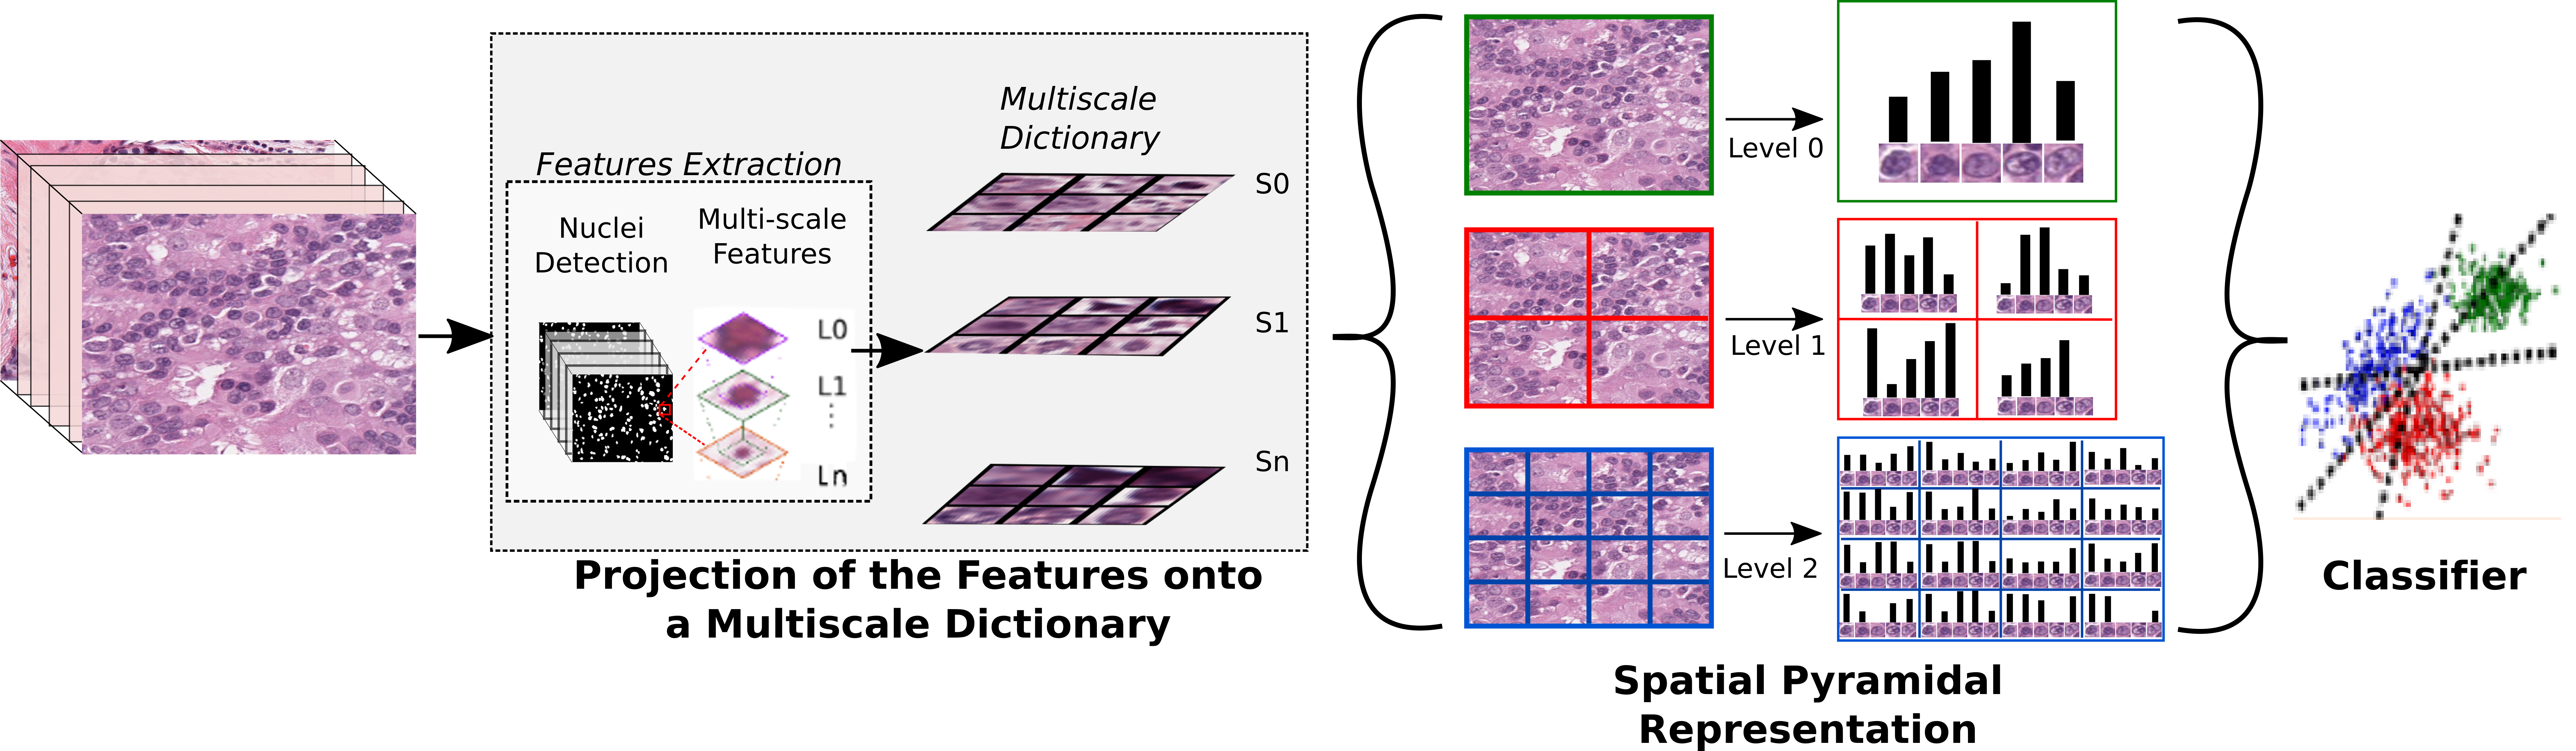
\includegraphics[width=\textwidth,heigth=15cm]{nuevoM/metodoSpatial.png}
    
% \end{frame}

\begin{frame}{Nuclei Detection}
    \centering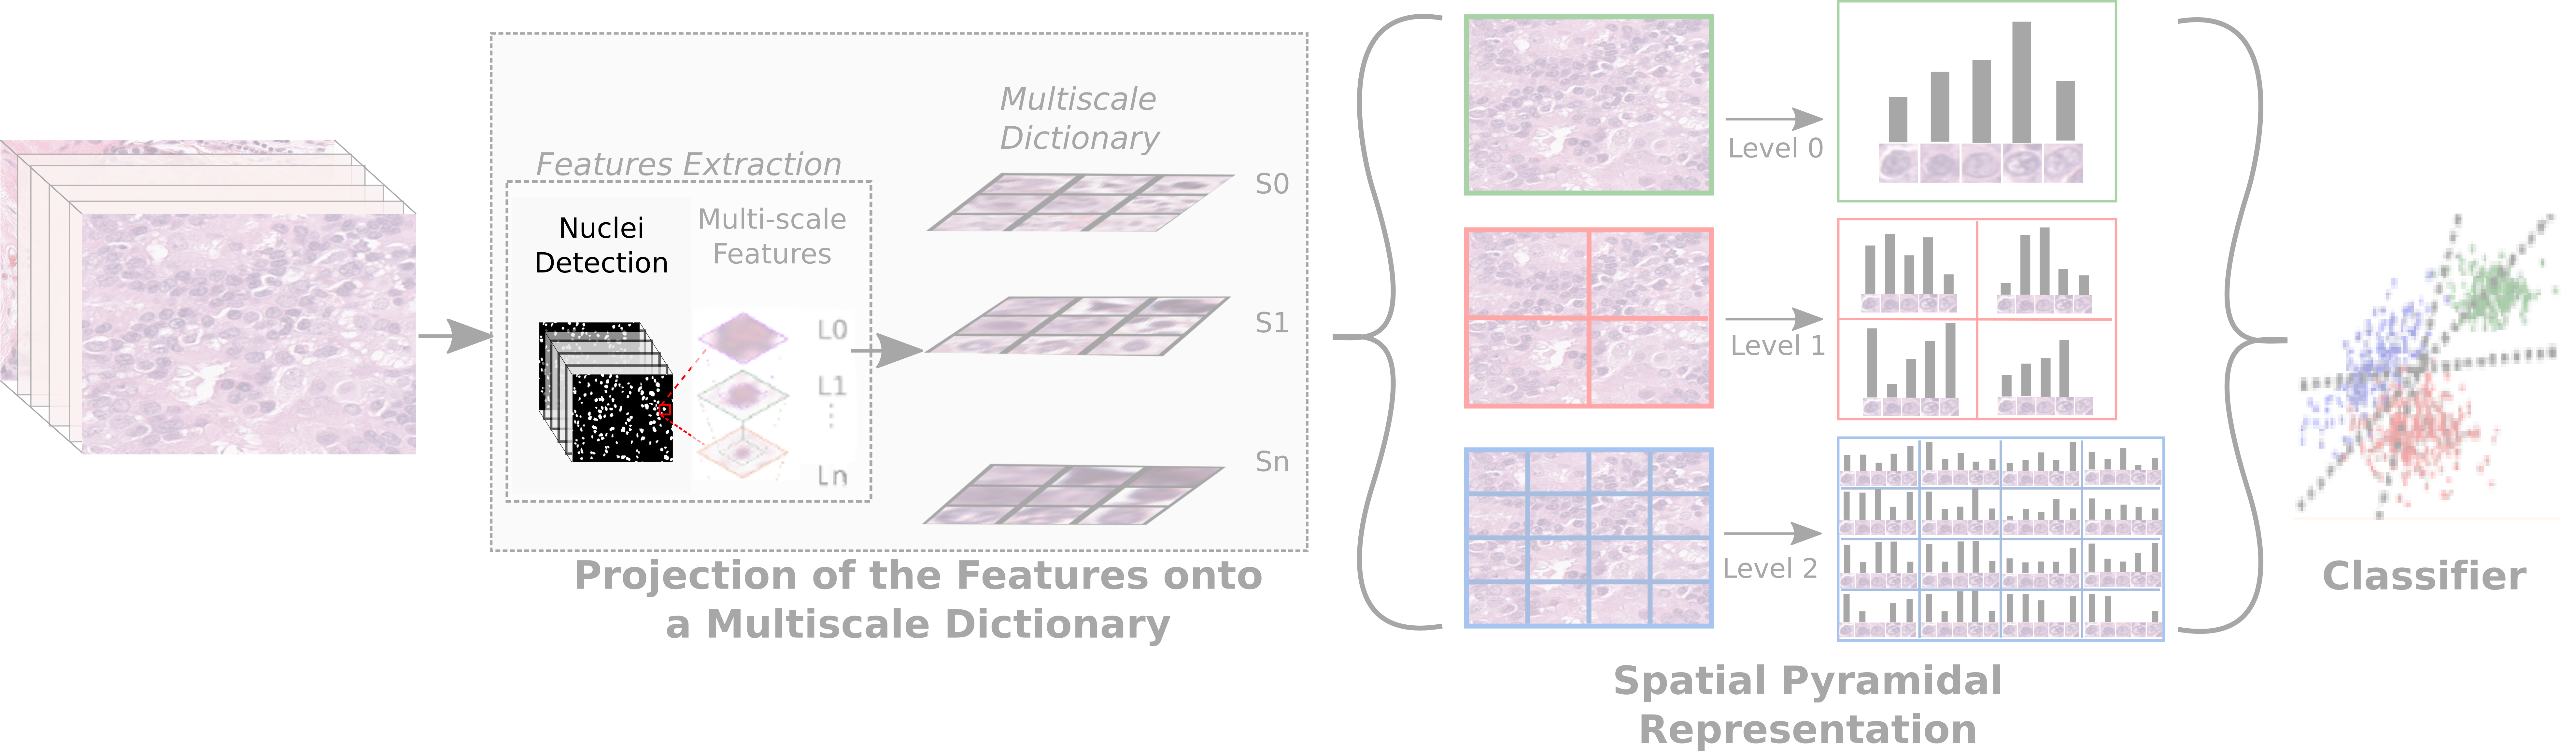
\includegraphics[width=\textwidth]{imagenes/nucleistep.png}
\end{frame}
\begin{frame}{Nuclei Detection}
%\hspace*{-3cm}
\LARGE
\begin{itemize}
\LARGE\item<1-> \small Using a color deconvolution technique the Hematoxylin (H) and eosin (E) stains are estimated \footnote{\tiny{A method for normalizing histology slides for quantitative analysis, Macenko et al.ISBI 2009}}
\item<3-> \small Watershed algorithm is used to detect nuclei candidates in H stain%\footnote{\tiny{Veta M.,ISBI 2011}}
\item<4-> \small Final candidates are found after morphological operations
\end{itemize}

\begin{textblock*}{2cm}(1cm,6cm) % {block width} (coords)
\begin{figure}
\includegraphics<1->[width=2cm]{MSER/1.jpeg}
\end{figure}
\end{textblock*}
\begin{textblock*}{2cm}(3.2cm,6cm) % {block width} (coords)
\begin{figure}
\includegraphics<2->[width=2cm]{MSER/2.jpeg}
\end{figure}
\end{textblock*}
\begin{textblock*}{2cm}(5.4cm,6cm) % {block width} (coords)
\begin{figure}
\includegraphics<3->[width=2cm]{MSER/3.jpeg}
\end{figure}
\end{textblock*}
\begin{textblock*}{2cm}(7.6cm,6cm) % {block width} (coords)
\begin{figure}
\includegraphics<4->[width=2cm]{MSER/4.jpeg}
\end{figure}
\end{textblock*}
\begin{textblock*}{2cm}(9.8cm,6cm) % {block width} (coords)
\begin{figure}
\includegraphics<5->[width=2cm]{MSER/5.jpeg}
\end{figure}
\end{textblock*}
\end{frame}


\begin{frame}{Multi-scale Feature Extractor}

\centering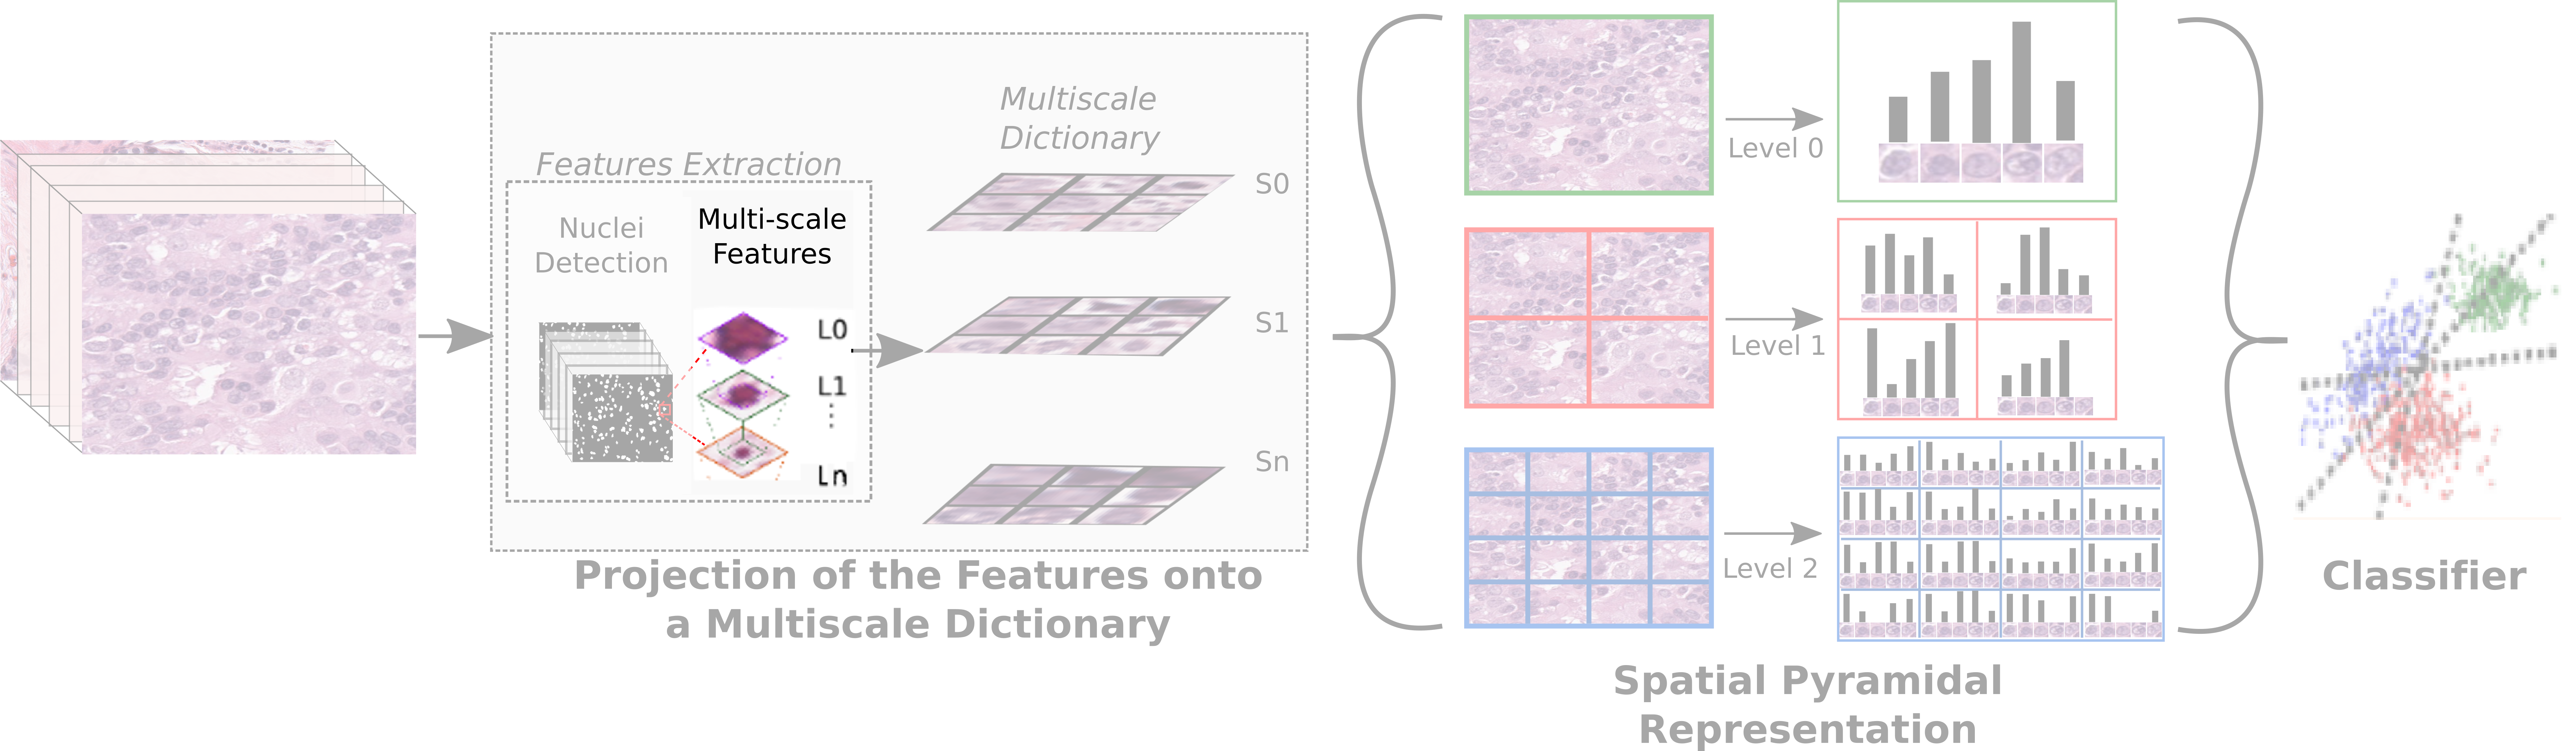
\includegraphics[width=\textwidth]{imagenes/featurestep.png}
    
\end{frame}


\begin{frame}{Multi-scale Feature Extractor}
 \begin{itemize}
     \item<1-> A Delaunay triangulation is built using the nuclei centroids (nodes) to determine directly connections
     \item<2-> Each nucleus is characterised by using their own information and relative measures of a representative nucleus obtained from the first order connected nuclei, using: mean, std, and  difference
     \item<3-> Haralalick features are extracted from each nucleus scale of a pyramidal decomposition
 \end{itemize}
\only<1>{\includegraphics[width=0.9\textwidth]{imagenes/delanoy.png}}
 \only<2>{\includegraphics[width=0.9\textwidth]{imagenes/delanoyANA2.png}}
\end{frame}

% \begin{frame}{Pyramidal Decomposition}
    
%     \item<1->\justifying The characterization of each nucleus was performed by analyzing multiple scales an extracting Haralicks Features in each scale
%     \item<2-> \justifying The feature vector corresponds to the information from Haralick features in each scale concatenated along one dimension.
%     \begin{figure}
%         \hspace{-1cm}\includegraphics<1->[width=7cm]{imagenes/descriptor.jpg}
%     \end{figure}
%     \begin{textblock}{20}(11,10)
%         \onslide<2->{$F(X_i)=\lbrace L0,L1,L2\rbrace$}
%     \end{textblock}
 
% \end{frame}


% \begin{frame}{Multi-scale Feature Extractor}
% \begin{itemize}
% \item<1->\justifying The characterization of each nucleus was performed by analyzing multiple scales an extracting Haralick Features in each scale
% \item<2->\justifying Also a realative measureThe characterization of each nucleus was performed by analyzing multiple scales an extracting Haralick's Features in each scale
% \item<2-> \justifying The feature vector corresponds to the information from RGB patches which are concatenated along one dimension.
% \end{itemize}
% \begin{figure}
% \hspace{-1cm}\includegraphics<1->[width=7cm]{imagenes/descriptor.jpg}
% \end{figure}
%  \begin{textblock}{20}(11,10)
%   \onslide<2->{$F(X_i)=\lbrace L0,L1,L2\rbrace$}
%  \end{textblock}
% \end{frame}

\begin{frame}{Multiscale Dictionary Building}
    \centering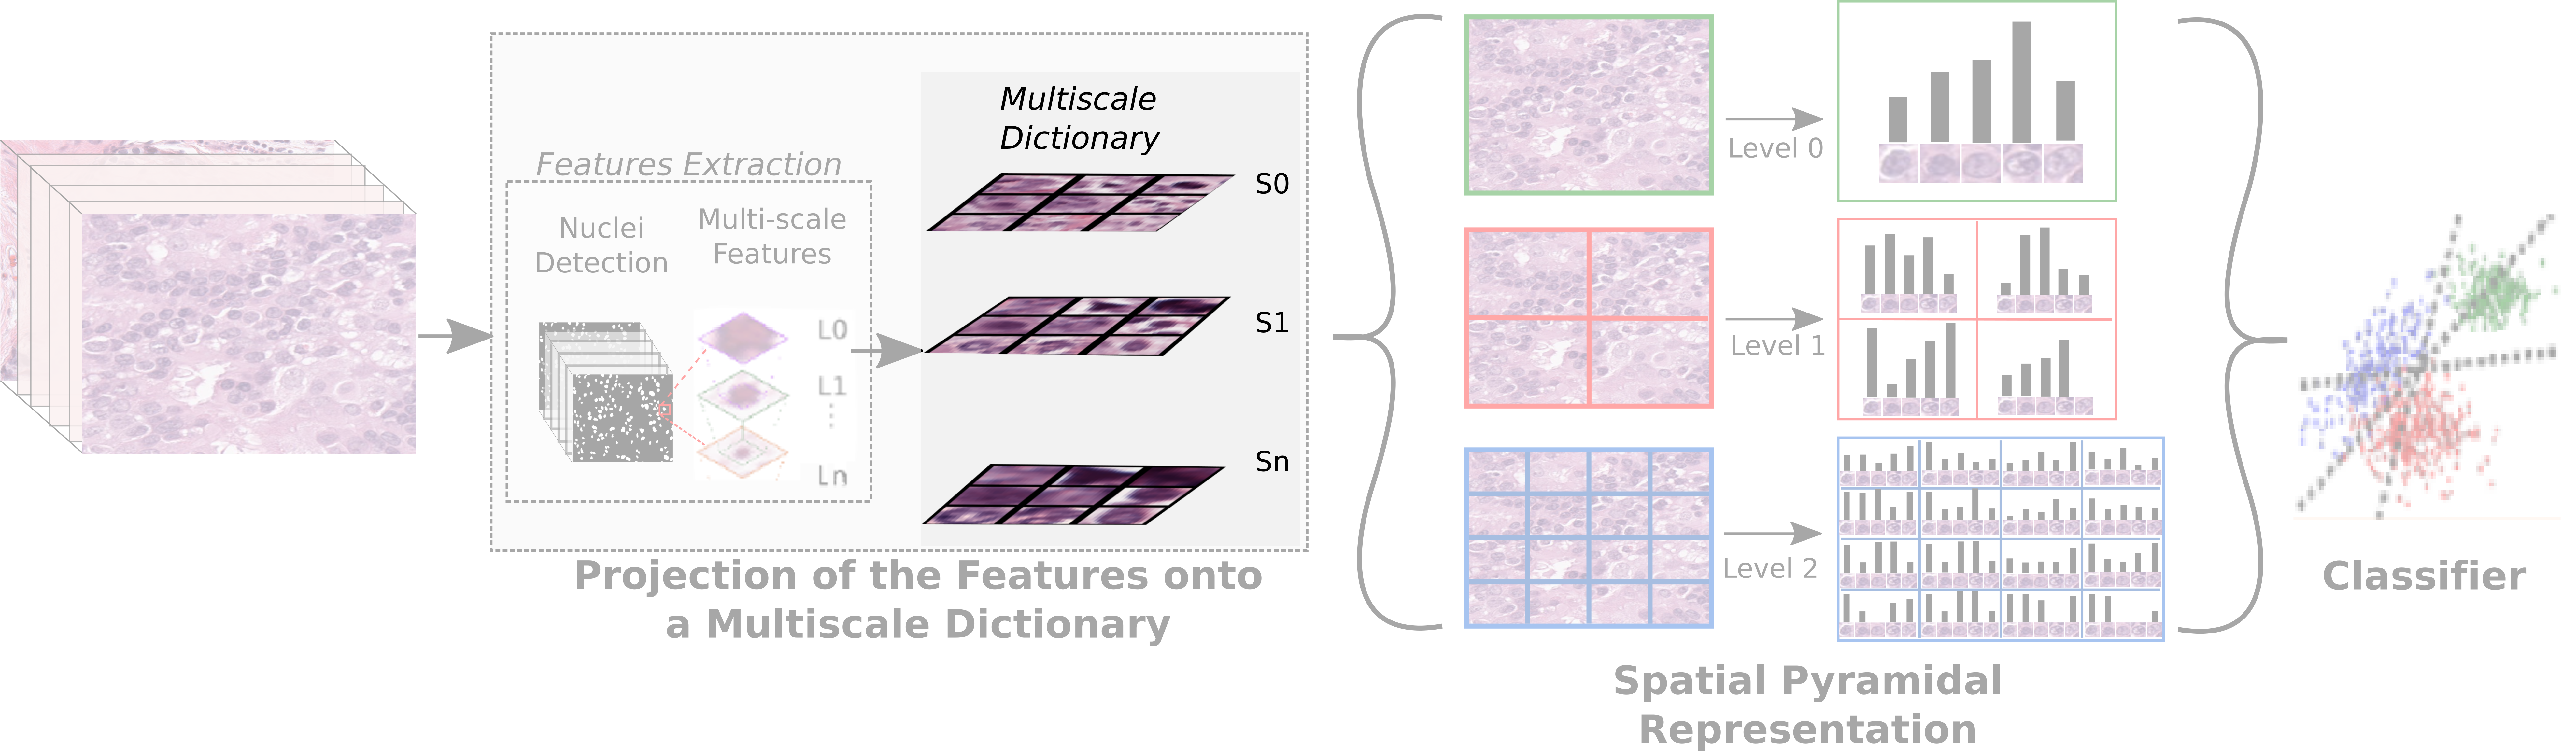
\includegraphics[width=\textwidth]{imagenes/dictionarystep.png}
\end{frame}

\begin{frame}{Multiscale Dictionary Building}
\centering\includegraphics[width=\textwidth]{nuevoM/dictionaryBuilding.png}
    
\end{frame}


%
%\begin{frame}{Multi-scale Features}
%\begin{itemize}
%\item<1->\justifying Each nucleus candidate is represented by multiple scales characterized by the discrete cosine transform (DCT) using enough coefficients to reconstructing the original image
%\item The coefficients from different scales are concatenated into a single feature  
%\end{itemize}
%\begin{figure}
%\hspace{-4.5cm}\includegraphics<1->[width=7cm]{imagenes/descriptor.jpg}
%\end{figure}
% \begin{textblock}{20}(9,10)
%  \onslide<2->{$F(X_i)=\lbrace DCT(L0),DCT(L1),DCT(L2)\rbrace$}
% \end{textblock}
%\end{frame}

\begin{frame}{Dictionay Building and histogram representation}
\begin{columns}
\begin{column}{4cm}
\begin{overprint}
\begin{figure}
\includegraphics<1>[width=0.95\textwidth]{dicc/kmeans.png}
%\includegraphics<2>[width=0.95\textwidth]{dicc/1.png}
\includegraphics<2>[width=0.95\textwidth]{dicc/2.png}
%\includegraphics<4>[width=0.95\textwidth]{dicc/3.png}
\includegraphics<3>[width=0.95\textwidth]{imagenes/unehistogram.png}
%\includegraphics<4>[width=0.95\textwidth]{imagenes/multiplehistogram.png}
\caption{\only<1>{K-means Algorithm}%\only<2>{Dictionary with L0}
%\only<3>{Dictionary with L1}
\only<2>{Decoded Dictionary Representation}
\only<3->{Ocurrence representation}}
\end{figure}
\end{overprint}
%\vspace{0.5cm} 
\end{column}
\begin{column}{8cm}
\begin{overprint}
\begin{itemize}
\item<1-> The multi-scale feature space is  partitioned with a $k$-means algorithm
\item<2-> Each centroid corresponds to a visual word of the Dictionary
\item<3-> An image is represented using their nuclei at different scales by counting the occurrences at the dictionary obtained a histogram.
\end{itemize}
\end{overprint}
\end{column}
\end{columns}
\end{frame}


\begin{frame}{Spatial Pyramidal Matching}
\centering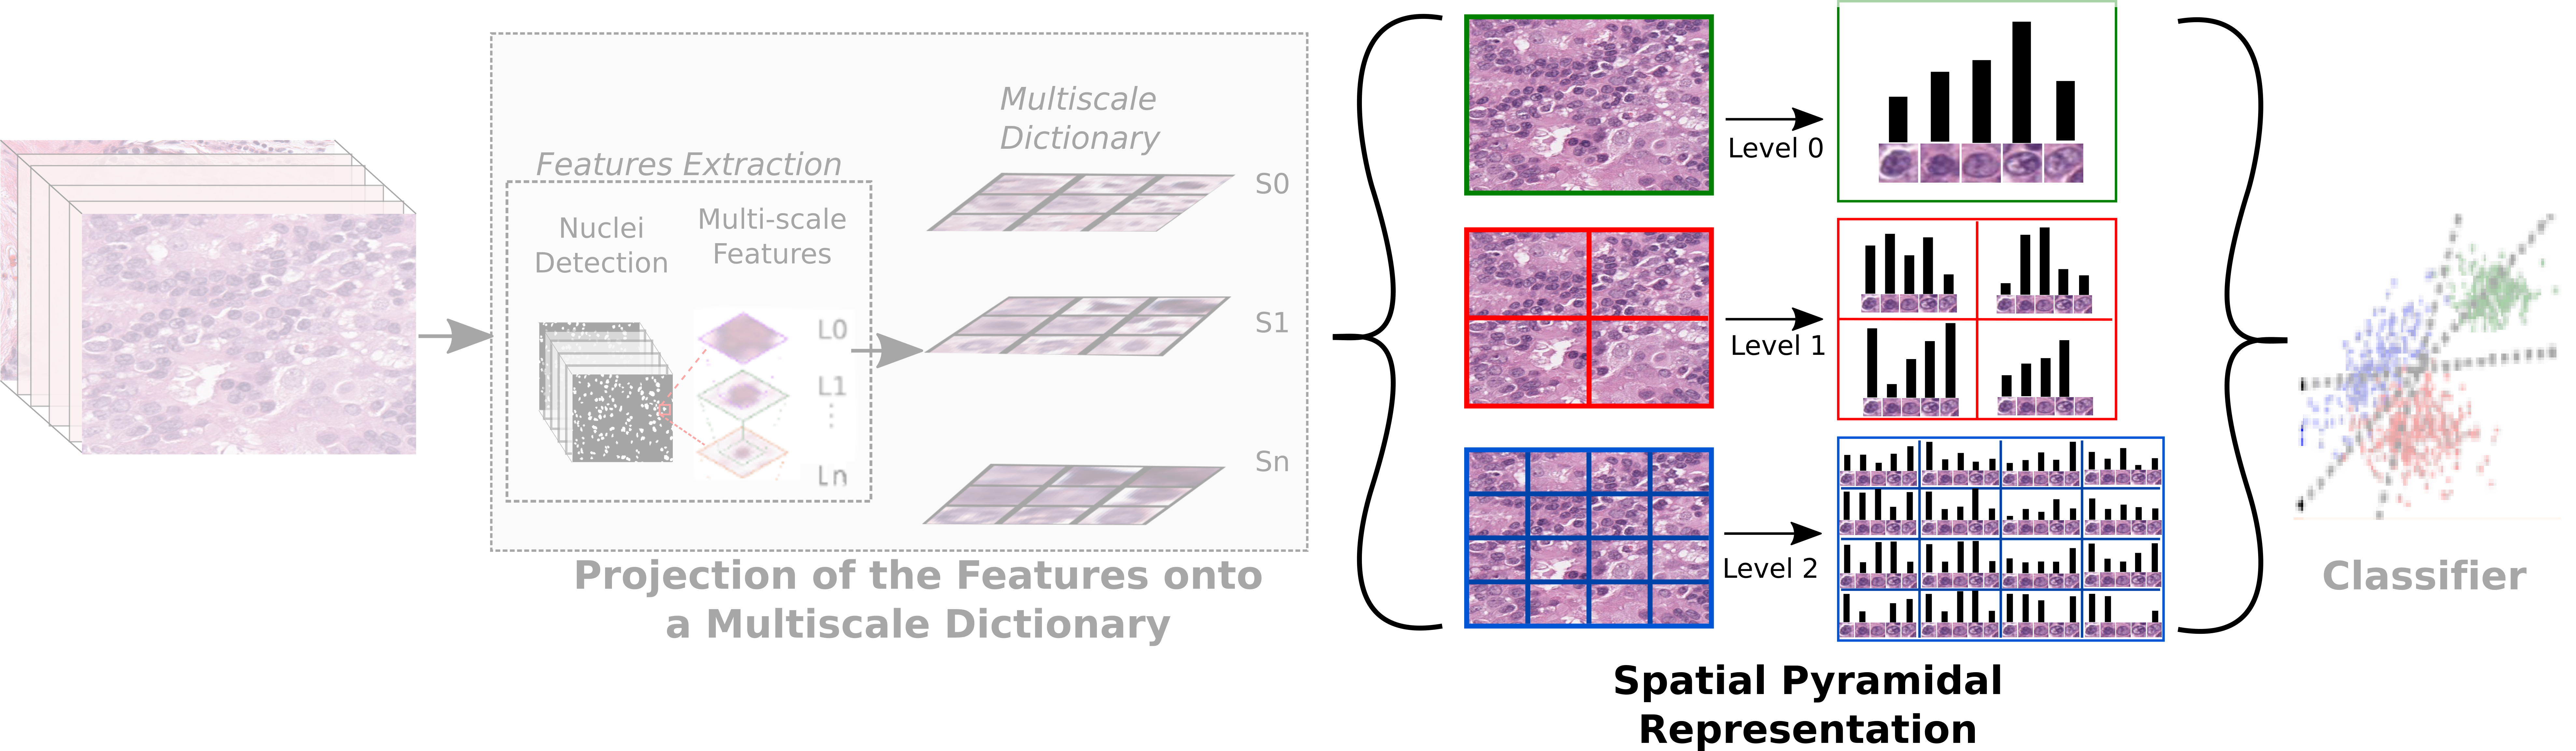
\includegraphics[width=\textwidth]{imagenes/pyramidalstep.png}
\end{frame}


\begin{frame}{Spatial Pyramidal Matching}
\only<1-2,6>{\vspace{-3.5cm}}
\begin{itemize}
\item<1-> Local representation at several levels of resolution using a bag of features approach

\item<2-> The construction is as follow:
\item<6> The histograms are concatenated into a single vector and feed the classifier
\end{itemize}

\centering\only<3>{\includegraphics[width = 0.6\textwidth]{imagenes/pyl0.png}}
\centering\only<4>{\includegraphics[width = 0.6\textwidth]{imagenes/pyl1.png}}
\centering\only<5>{\includegraphics[width = 0.6\textwidth]{imagenes/pyl2.png}}
\centering\only<6>{$f(Y)=[Hist(l0),hist(l1),hist(l2)]$}

\end{frame}

\begin{frame}{Second Approach using coded nuclei patches}

\includegraphics[width = \textwidth]{imagenes/newproposalSP.png}



\end{frame}

\begin{frame}{Nuclei Patches And Dimensionality Reduction}
\begin{itemize}
\item<1-> Patches of $n \times n $ pixels around all candidate nuclei are extracted

\item<2-> A convolutional neural network is trained to learn coded nuclei representations in a unsupervised way (auto-encoder)

\end{itemize}


\only<1->{\centering\includegraphics[width=0.8\textwidth]{imagenes_cnn/autoencoderNuclei.png}}

\end{frame}

\begin{frame}{Clustering Step}
\begin{itemize}
 \item The proposed deeplearning architecture\footnote{Guo et al., ICONIP17 } \normalsize minimize the reconstruction loss of the autoencoder and the clustering loss
 \item Intends to preserve the structure of the data
\end{itemize}
\includegraphics[width = \textwidth]{imagenes/ClusterinLayer.png}

\end{frame}






% \begin{frame}{Convolutional Neural Networks Baseline Framework  (CNN)}
%     \centering
%     \includegraphics[width=1\textwidth]{imagenes_cnn/CCn_methodF.png}
 
% \end{frame}

% \begin{frame}{CNN Baseline Framework}
% \begin{itemize}
%  \item The Image is divided in several patches
%  \pause
%  \item A Data augmentation step is performed

%  \pause \item Different CNN were trained (VGG16, Alexnet, Resnet50, CNN) one at time
%   \pause\item The activation output is used as a feature vector of the patch and then is concatenated with the subsequents to obtain a feature vector of the whole image
%   \pause \item The feature vector is used to feed a classifier
% \end{itemize}
% \end{frame}

\section{Experiments and Results}

\begin{frame}{Experiments }
\begin{itemize}
\item  Mitos Atypia 14 public database was used
\item Combinations of binary classifications were evaluated to find which sets-up are best for different NP grade
\item  Patches of 92x92 pixels are extracted using the nuclei centroid as a seed
\item Different combinations of levels of SPYA framework were evaluated
\item Reduction of $2\times$ was selected to bottle neck.


 
\end{itemize}

\end{frame}



\begin{frame}{Dataset- Mitos Atypia 14}

\begin{table}[]
\begin{tabular}{|m{1cm}|m{2cm}|}
\hline
%Grade &\centering  \#40X images &\centering Total Patches 344x344 pixels&\centering  Train & Validation \\ \hline
\multicolumn{2}{|c|}{Original} \\ \hline  \hline
\centering
Grade & #40X images  \\ \hline
NP 1  & 92   \\ \hline
NP 2  & 900\\ \hline
NP 3  & 208   \\ \hline
\end{tabular}
\caption{Training and validation - 11 cases for training}
\end{table}
    \begin{table}[]
\begin{tabular}{|c|c|}
\hline
Grade & \# 40X images \\ \hline
NP 1  & 152           \\ \hline
NP 2  & 252           \\ \hline
NP 3  & 92            \\ \hline
\end{tabular}
\caption{Test dataset - 5 cases}
\end{table}
\end{frame}    
    
\begin{frame}{Autoencoder reconstruction}
\centering\includegraphics[width=0.4\textwidth]{imagenes_cnn/reconstruction.png}
    \\(a) Original patches dim(8464),(b)reconstruction from 4232 dim, (c) reconstruction from  1000 dim
\end{frame}


% \begin{frame}{Dataset- Mitos Atypia 14}

% \begin{table}[]
% \begin{tabular}{|m{1cm}|m{2cm}|m{3cm}|m{1.3cm}|m{1.3cm}|}
% \hline
% %Grade &\centering  \#40X images &\centering Total Patches 344x344 pixels&\centering  Train & Validation \\ \hline
% \multicolumn{2}{|c|}{Original} & \multicolumn{3}{c|}{After Augmentation} \\ \hline  \hline
% \centering
% Grade &\centering  \#40X images &\centering Total Patches 344x344 pixels&\centering  Train & Validation \\ \hline
% NP 1  & 92            & 21,344  &   18,144   & 3,200          \\ \hline
% NP 2  & 900           & 22,500  &  19,096    & 3,404     \\ \hline
% NP 3  & 208           & 20,800  &  17,764    & 3,036     \\ \hline
% \end{tabular}
% \caption{Training and validation - 11 cases for training}
% \end{table}
%     \begin{table}[]
% \begin{tabular}{|c|c|}
% \hline
% Grade & \# 40X images \\ \hline
% NP 1  & 152           \\ \hline
% NP 2  & 252           \\ \hline
% NP 3  & 92            \\ \hline
% \end{tabular}
% \caption{Test dataset - 5 cases}
% \end{table}
% \end{frame}    
    


\begin{frame}{Results using F1-Score}

The F-score is used to evaluate the classification
\begin{equation}
    F_{\beta} = (1+\beta^{2}).\frac{precision.recall}{(\beta^{2}.precision)+recall}
\end{equation}
$\beta=1$ is used this is the harmonic mean between precision and recall
\end{frame}




\begin{frame}{Results - BoF multiscale features, raw block}

\begin{table}
\begin{tabular}{|l|l|l|l|}
\hline
  & BOF PY & BOF PY L0 & BOF PY L1 \\ \hline
3 Vs. 1 and 2 & \textbf{0.624}   & 0.593 & 0.583 \\ \hline
1 Vs. 2 and 3 & \textbf{0.692} & 0.642  & 0.678 \\ \hline
1 Vs 2        & 0.650  & \textbf{0.713} & 0.660 \\ \hline
2 Vs 3        & 0.722 & 0.660  & \textbf{0.729} \\ \hline
1 Vs 3        & 0.628  & 0.675                           & \textbf{0.740} \\ \hline
\end{tabular}
\end{table}




\end{frame}

\begin{frame}{Results - Autoencoder Approach (non multiscale)}

\begin{table}[]
\begin{tabular}{|l|l|l|l|l|}
\hline
Task & SPYA   & SPYA L0 & SPYA L1 & SPYA L2                      \\ \hline
3 Vs. 1 and 2 & 0.659 &\textbf{ 0.700} & 0.619  & \multicolumn{1}{l|}{0.646}  \\ \hline
1 Vs. 2 and 3 & \textbf{0.544} & 0.508 & 0.527  & \multicolumn{1}{l|}{0.568} \\ \hline
1 Vs 2        & 0.532 & 0.446 & 0.520  & \multicolumn{1}{l|}{\textbf{0.545}} \\ \hline
2 Vs 3        & 0.612 & \textbf{0.664} &0.628  & \multicolumn{1}{l|}{ 0.595} \\ \hline
1 Vs 3        & \textbf{0.639} & 0.557 & 0.588  & \multicolumn{1}{l|}{0.622} \\ \hline
\end{tabular}
\caption{Results using a coded representation of the nuclei}
\end{table}

\end{frame}




% \begin{frame}{Results - Autoencoder Approach OLD}

% \begin{table}[]
% \begin{tabular}{|l|l|l|l|l|}
% \hline
% Task & SPYA   & SPYA L0 & SPYA L1 & SPYA L2                      \\ \hline
% 3 Vs. 1 and 2 & 0.578 & \textbf{0.630} & 0.565  & \multicolumn{1}{l|}{0.530}  \\ \hline
% 1 Vs. 2 and 3 & \textbf{0.624} & 0.564 & 0.520  & \multicolumn{1}{l|}{0.489} \\ \hline
% 1 Vs 2        & 0.473 & \textbf{0.597} & 0.542  & \multicolumn{1}{l|}{0.573} \\ \hline
% 2 Vs 3        & 0.560 & 0.603 &0.606  & \multicolumn{1}{l|}{ \textbf{0.632}} \\ \hline
% 1 Vs 3        & 0.623 & \textbf{0.716} & 0.639  & \multicolumn{1}{l|}{0.632} \\ \hline
% \end{tabular}
% \caption{Results using a coded representation of the nuclei}
% \end{table}

% \end{frame}


% \begin{frame}{Results of CNN Baseline}
% \begin{table}[]
% \begin{tabular}{|p{1.5cm}|p{1.4cm}|p{1.3cm}|p{1.3cm}|p{1.3cm}|p{1.3cm}|}
% \hline
%               & CNN (1024dim)  & CNN (3dim)     & VGG16 & Alexnet & Resnet50       \\ \hline
% 3Vs.1 and 2 & 0.635          & 0.523          & 0.629 & 0.493  & \textbf{$0.645\pm0.037$} \\ \hline
% 1Vs.2 and 3 & \textbf{0.676} & 0.645          & 0.564 & 0.581  & $0.553\pm0.05$          \\ \hline
% 1 Vs 2        & 0.637         & \textbf{0.664} & 0.453 & 0.623   & $0.582\pm0.04$         \\ \hline
% 2 Vs 3        & 0.570          & 0.567          & 0.544 & 0.619   & \textbf{$0.670\pm0.046$} \\ \hline
% 1 Vs 3        & 0.666         & \textbf{$0.642\pm0.041$} & 0.620 & $0.649\pm0.038$   & $0.563\pm0.034$          \\ \hline
% \end{tabular}
% \end{table}    



% \end{frame}



% \begin{frame}{Results of BoF multiscale descriptor}
% \begin{table}[]
% \begin{tabular}{|c|c|c|}
% \hline
% Experiment/S.Patch & \begin{tabular}[c]{@{}c@{}}32x32\\ L2\end{tabular} & \begin{tabular}[c]{@{}c@{}}20x20\\ L2\end{tabular} \\ \hline
% 1 vs 2 and 3       & \textbf{0.593}                                              & 0.434                                              \\ \hline
% 3 vs 1 and 2       & \textbf{0.642}                                              & 0.47                                               \\ \hline
% 1 vs 2             & \textbf{0.7128}                                             & 0.47                                               \\ \hline
% 1 vs 3             & 0.660                                              & \textbf{0.7029}                                             \\ \hline
% 2 vs 3             & \textbf{0.6759}                                             & 0.5813                                             \\ \hline
% \end{tabular}
% \caption{Results Bag Of Features}
% \end{table}

% \end{frame}


% \begin{frame}{Visual Performance of the Autoencoder}


%     \centering
%     \includegraphics[width=0.85\textwidth]{imagenes_cnn/autoencoderresponse.png}
%     \\Autoncoder Reconstruction


% \end{frame}


% \begin{frame}{Final Remarks}

% \begin{itemize}
%     \item The Slightly variation between the NP grades and the high tissue variability makes it challenging to find an adequate model
%     \item The CNN model could be improved if take advantage of the spatial information
%     \item The auto-encoder representation and vocabulary construction maybe are not the most accurate
% \end{itemize}
    
% \end{frame}


% \begin{frame}{Current Work}

% \begin{itemize}
%   \item To determine a better cluster representation 
  
%   \item To evaluate the frameworks in a new database
  
%   \item To determine if there exists a relationship between NP grading and the cancer recurrence (Future work)
% \end{itemize}

% \end{frame}


\begin{frame}{Final remarks}

\begin{itemize}
    \item This work intended to establish an objective difference between the three NP grades and the possibility to use it in the pathologist workflow 
    \item The multi-scale representation have an impact on the performance of the classification task using only first order relationships
    \item The use of the dimensional reduction preserves the latent space but without improve the classification task, not yet!.
\end{itemize}
    
\end{frame}

\begin{frame}{New Dataset}

\begin{itemize}
\item 24 cases of DCIS from Sunnybrook Health Institute
\item 306 marked regions from 24 cases grading by an expert pathologist 
\end{itemize}
    \begin{table}[]
\begin{tabular}{|c|c|}
\hline
Grading              & \# Marked Areas \\ \hline
Grade 1              & 135             \\ \hline
Grade 2              & 132             \\ \hline
Grade 3              & 39              \\ \hline\hline
\textbf{Total Cases} & \textbf{24}     \\ \hline
\end{tabular}
\end{table}
\end{frame}





%
%
%
%\begin{frame}{Results}
%
%\begin{table}[l]
%\begin{tabular}{|m{1.2cm}|m{1cm}|m{1cm}|m{1cm}|m{1cm}||m{1cm}|m{1cm}|m{1cm}|}
%\hline
%              & PS.  & PS L0   & PS L01 & PS L2 & BOF PY          & BOF PY L0       & BOF PY L1\\ \hline
%3 Vs. 1 and 2 & 0.578     & \textbf{0.630} & 0.565        & 0.53         & 0.624          & 0.593           & 0.583\\ \hline
%1 Vs. 2 and 3 & 0.624    & 0.564          & 0.520         & 0.489        & \textbf{0.692} & 0.642           & 0.678\\ \hline
%1 Vs 2        & 0.473     & 0.597          & 0.542         & 0.573        & 0.650           & \textbf{0.713} & 0.660\\ \hline
%2 Vs 3        & 0.560     & 0.603          & 0.606         & 0.632        & 0.722          & 0.660           & \textbf{0.729}\\ \hline
%1 Vs 3        & 0.623     & 0.716          & 0.639         & 0.632       & 0.628          & 0.675         & \textbf{0.740} \\ \hline
%\end{tabular}
%\end{table}
%    
%\end{frame}
%
%
%
%\begin{frame}{CNN Framework}
%    \centering
%   \includegraphics[width=1\textwidth]{imagenes_cnn/CCn_methodFS2.png}
%\end{frame}
%










% \begin{frame}{Results}

% \begin{table}[]
% \begin{tabular}{|l|l|l|l|}
% \hline
% Experiment  & Validation  & test patches & FOV on test \\ \hline
% CNN 1       & 0.78           & 0.266                & 0.482                          \\ \hline
% CNN 2       & 0.8345         & 0.290                & 0.53                           \\ \hline
% Fully CNN   & 0.3481         &                      &                                \\ \hline
% Khan et al. & 0.845(k-fold)          &                      & \textbf{0.71}*                  \\ \hline
% BoF         &                &                      & 0.66 *                          \\ \hline
% \end{tabular}
% \caption{Accuracy - * 11 cases for train, 5 for test}
% \end{table}
% \end{frame}



%
%\begin{frame}{}
%\includegraphics[width=\textwidth]{imagenes/ResultACCepoch.png}
%    
%\end{frame}

%\begin{frame}{Confusion Matrix}
%
%\begin{table}[]
%\begin{tabular}{|c|c|c|}
%\hline
%51 & 97  & 4  \\ \hline
%17 & 195 & 40 \\ \hline
%5  & 67  & 20 \\ \hline
%\end{tabular}
%\caption{for CNN2}
%\end{table}
%    
%\end{frame}





\begin{frame}{Dataset pre-processing}

\begin{itemize}
    \item<1-> Existing tile extraction algorithm was modified to form a grid from the region marked instead of a regular grid in build from the (0,0) cords
    \item<2-> 1698 new tiles of $1024\times1024$ are obtained
\end{itemize}

\begin{columns}
\begin{column}{0.5\textwidth}
\includegraphics[width=\textwidth]{nuevoM/oldalgo.png}\\
\centering \small  Old Extraction - Forms Tiles with large empty areas
\end{column}
\begin{column}{0.5\textwidth}
\includegraphics[width=\textwidth]{nuevoM/newalgo.png}\\
\centering \small New Extraction - Tiles with less of $50\%$ of ROI are discarded
\end{column}
\end{columns}
    
\end{frame}



\begin{frame}{Future Work}

\begin{itemize}
    \item To compute the dispersion in the different classification task
    \item To use second order relationships
    \item To validate the approaches in a new dataset
    \item To compare the results with the state of the art
     
\end{itemize}
    
\end{frame}

\section{MicroMetastasis Project}

%\subsection{Sentinel Lymph Node}

\begin{frame}[fragile]{\textbf{Sentinel Lymph Node}}
\only<2> {\vskip-1cm}
\begin{columns}
   \column{0.50\textwidth} 
 \only<1->{\flushleft{\vspace{-5mm}\includegraphics[height=6cm,width=5cm]{imagenes2/Imagen2.png} }}
 \raggedleft
 \column{0.35\textwidth}
\only<1->{ \\

    \begin{itemize}
    \item<1-> \large Lymph nodes are important to determine if the cancerous cells have acquired the capacity to disseminate to other body parts. 
    %Lymph nodes determine if the cancerous cells have acquired the capacity of disseminating to other body part.
    %The lymph nodes are important to help to determine if the cancerous cells have acquired the capacity of disseminating to other body parts.
    \end{itemize}}

\end{columns}
\only<2>{\\
  \Centering   
 \vspace{-30mm} \begin{block}{}
 
\large A sentinel lymph node is defined as the {\textcolor{violeta}{\textbf{\Large first lymph node}}}  where cancer cells are most likely to spread from a primary tumor
   %This is the first node lymph closest to the tumor.
    \end{block}}   

\end{frame}
%-------------------------------------------

%\subsection{Types Metastasis}
%---------------------------------
\begin{frame}{\textbf{Sentinel Metastasis Types}} {\textbf{Type of nuclei}}
\large A biopsy procedure aims to determine if there are node cancerous cells
\begin{figure}
    \centering
    \includegraphics[height=5cm,width=13cm]{imagmetodo/nucleitypes.png}
    
\end{figure}
 \begin{block}
   
{\textcolor{mDarkTeal}{\textbf{\large PLEOMORPHISM:}}} Color, Area and texture.
    \end{block}
\end{frame}
%---------------------------------

\begin{frame}[fragile]{\textbf{Sentinel Metastasis Types }}
%A Sentinel Lymph Node Biopsy is a procedure in which the Sentinel Lymph Node is identified, removed and examined to determine if there are cancerous cells.


\begin{figure}
    \centering
   \includegraphics[width=1\textwidth ]{imagenes2/types.png} 
    \label{fig:my_label}
\end{figure}


 
 % the macro-metastses diameter is larger than 2 mm 
 % the micro-metastases diameter is between 0.2mm and 2 mm
 %and the isolated tumor cells are smaller than 0.2mm... The expert only can find  one or two tumoral cell in the WSI  .  

  
\end{frame}
%-------------------------------------------------

%-------------------------------------------------------
\section{\large Research Problem}

%-------------------------------------------------------
%\subsection{Research Problem }
\begin{frame}{}
%\transduration{0.75}

%-------------------------------------------------------


\only<1->{\vspace*{+1cm}\begin{block}{Research Problem}

“The sentinel lymph node is the most likely lymph node to contain metastasized cancer cells and is excised, histopathologically processed, and examined by a pathologist. \textcolor{morado} {\textbf {This tedious examination process is time-consuming and can lead to small metastases being missed” }}. \footnotemark[2]

 \end{block}}
 

\only<2>{
\begin{block}{Hypothesis}
It is possible to localize any metastases in the whole slide image from features extracted from groups of metastases learned from other images with the presence of metastases. 

%by determining groups of them from extracted characteristics learned of others images with metastases.%If I extract characteristics of the nuclei I can determine by means of the classification to which cells they belong.
% 
%it is possible to locate any metastasis in the wsi from features extracted from groups of metastases learned from other images with the presence of metastases.
 \end{block}}
 \footnotetext[2]{\tiny Geert Litjens, Peter Bandi, Babak Ehteshami Bejnordi, Oscar Geessink, Maschenka Balkenhol, Peter Bult, Altuna Halilovic, Meyke Hermsen, Rob van de Loo, Rob Vogels, Quirine F Manson, Nikolas Stathonikos, Alexi Baidoshvili, Paul van Diest, Carla Wauters, Marcory van Dijk, Jeroen van der Laak; 1399 H \& E-stained sentinel lymph node sections of breast cancer patients: the CAMELYON dataset, GigaScience, Volume 7, Issue 6, 1 Jñune 2018, giy065, https://doi.org/10.1093/gigascience/giy065}
\end{frame}

%-------------------------------------------------------
\section{\large Methodology}
\begin{frame}{\textbf{Methodology}}
%-------------------------------------------------------
\vspace{-0.7cm}
\begin{figure}
    \centering
   \includegraphics[height=9cm,width=14cm]{imagenes3/metodologia1.png}
  
\end{figure}
  
% my proposed methodology is:
% first and pre-processing step , then Nuclei Detection later Feature extraction and finally plsa clustering.

\end{frame}
%---------------------------------------

\begin{frame}{\textbf{Pre-Processing }}

\vspace{-0.5cm}
\begin{figure}
    \centering
  \includegraphics[height=9cm,width=14cm]{imagenes3/medotologia2.png}
   
\end{figure}

     
     % in this step i extract patches of  n by n  pixels 
\end{frame}
%------------------------------------------------------
\begin{frame}{\textbf{Pre-Proccesing}}
\begin{columns}
   \column{0.3\textwidth}
   \begin{figure}
    \centering
    \includegraphics[height=4cm,width=4cm]{imagmetodo/WSItotal.PNG}
    \caption*{\large WSI}
    \end{figure}
    
    \column{0.1\textwidth}
     \begin{figure}
         \centering
         \includegraphics[height=0.5cm,width=0.5cm]{imagenes3/flecha.png}
         \end{figure}
         
      \column{0.3\textwidth}   
         \begin{figure}
             \centering
             \includegraphics[height=4cm,width=4cm]{imagmetodo/segmentidentify.PNG}
             \caption*{\large Expert segmentation}
         \end{figure}
         
          \column{0.1\textwidth}
     \begin{figure}
         \centering
         \includegraphics[height=0.5cm,width=0.5cm]{imagenes3/flecha.png}
         \end{figure}
         
         \column{0.3\textwidth}
         \begin{figure}
             \centering
             \includegraphics[height=4cm, width=4cm]{imagmetodo/patient_012_node_0_0_33.jpg}
             \caption*{\centering \large Samples \\ \small ($1024 \times 1024$ pixels)}
         \end{figure}
    \end{columns}
\end{frame}

%----------------------------------------------------------------
\begin{frame}{\textbf{Feature Extraction }}
% the third step is feature extraction .

  \vspace{-0.5cm}
\begin{figure}

    \centering
  \includegraphics[height=9cm,width=14cm]{imagenes3/metodologia3.png}
   
\end{figure}
\end{frame}
%%---------------------------------------------
\begin{frame}{\textbf{Feature Extraction}}  {\large Color Space }

\large The color space (RGB) of  each image.
\\
\centering
\vspace{2mm} \animategraphics[controls, height=5.5cm,width=13cm,step]{}{imagenes3/graficos/color}{1}{3}
    
\end{frame}
%%-------------------------------------------
\begin{frame}{\textbf{Feature Extraction}} {\large Projection to the (R-B,G plane}
Project the (r, g, b)  to the [(r -b), g] plane, where relative differences
among Hematoxylin–eosin colours are highlighted.
\\
\centering
\vspace{2mm} \animategraphics[controls, height=5.5cm,width=13cm,step]{}{imagenes3/graficos/rb}{1}{3}
   
\end{frame}
%%------------------------------------------
\begin{frame}{\textbf{Feature Extraction}} {\large Characterization of the projection}

 The G axis is divided into a set of intervals and histograms per interval are computed.

\only <1-2> {\vskip-0.5cm} 
\begin{columns}

\column{0.3\textwidth}   

  \only<1-2>{\begin{figure}
 \centering
    \includegraphics[heigth=0.2cm, width= 11cm]{imagenes3/graficos/histograma.png}
    
\end{figure}}

\column{0.3\textwidth}
\only <2>{{\vskip -2cm}
\begin{block}{Statistics per  Histogram}
\begin{itemize}
    \item Mean
    \item Variance
    \item Skewness
    \item Kurtosis
\end{itemize}
\end{block}}

\end{columns}

\only <3->{ 
\begin{figure}
    \centering
 \includegraphics[heigth=0.7cm, width= 12cm]{imagenes3/graficos/vector.png}
\end{figure}}
\end{frame}

\end{document}